

% generated by Plantuml 1.2022.7       
\definecolor{plantucolor0000}{RGB}{241,241,241}
\definecolor{plantucolor0001}{RGB}{24,24,24}
\definecolor{plantucolor0002}{RGB}{173,209,178}
\definecolor{plantucolor0003}{RGB}{0,0,0}
\definecolor{plantucolor0004}{RGB}{3,128,72}
\definecolor{plantucolor0005}{RGB}{132,190,132}
\definecolor{plantucolor0006}{RGB}{242,77,92}
\definecolor{plantucolor0007}{RGB}{200,41,48}
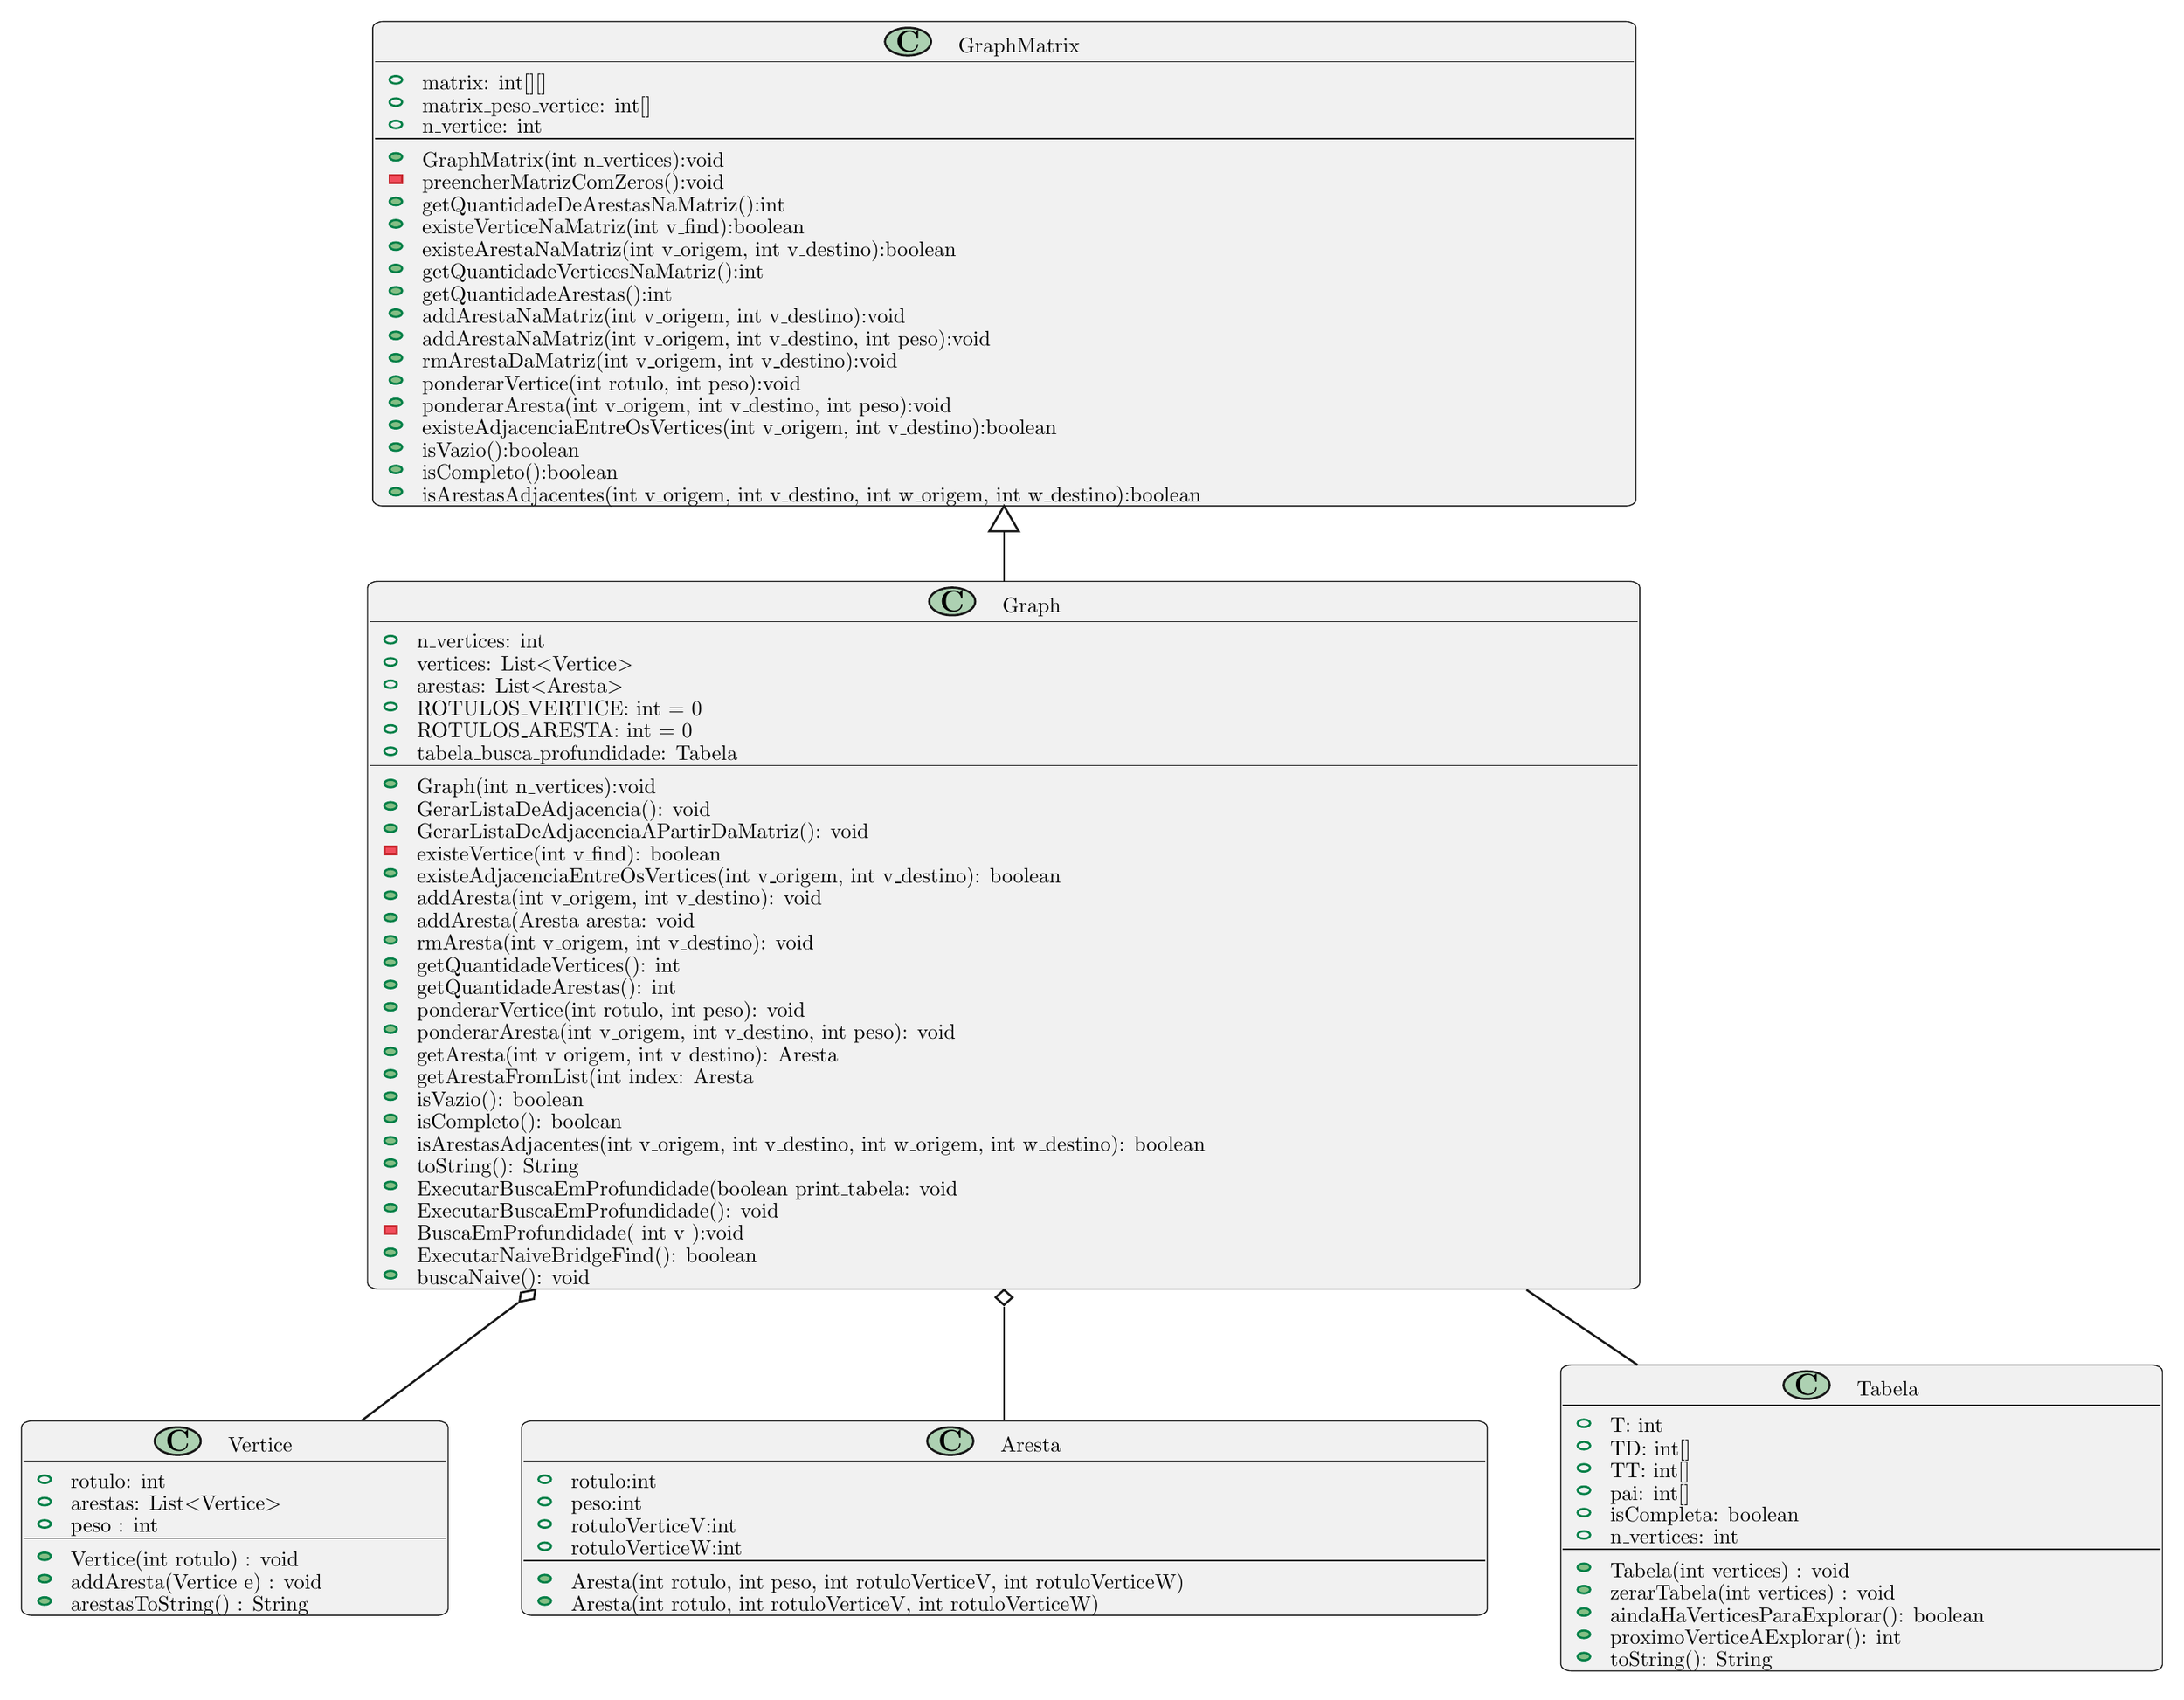
\begin{tikzpicture}[yscale=-0.6
,pstyle0/.style={color=plantucolor0001,fill=plantucolor0000,line width=0.5pt}
,pstyle1/.style={color=plantucolor0001,fill=plantucolor0002,line width=1.0pt}
,pstyle2/.style={color=plantucolor0001,line width=0.5pt}
,pstyle3/.style={color=plantucolor0004,line width=1.0pt}
,pstyle4/.style={color=plantucolor0004,fill=plantucolor0005,line width=1.0pt}
,pstyle5/.style={color=plantucolor0007,fill=plantucolor0006,line width=1.0pt}
,pstyle6/.style={color=plantucolor0001,line width=1.0pt}
]
\draw[pstyle0] (174.5pt,12pt) arc (180:270:5pt) -- (179.5pt,7pt) -- (771.8193pt,7pt) arc (270:360:5pt) -- (776.8193pt,12pt) -- (776.8193pt,387.1758pt) arc (0:90:5pt) -- (771.8193pt,392.1758pt) -- (179.5pt,392.1758pt) arc (90:180:5pt) -- (174.5pt,387.1758pt) -- cycle;
\draw[pstyle1] (429.7097pt,23pt) ellipse (11pt and 11pt);
\node at (429.7097pt,23pt)[]{\textbf{\Large C}};
\node at (450.2097pt,14.127pt)[below right,color=black]{GraphMatrix};
\draw[pstyle2] (175.5pt,39pt) -- (775.8193pt,39pt);
\draw[pstyle3] (185.5pt,53.373pt) ellipse (3pt and 3pt);
\node at (194.5pt,43pt)[below right,color=black]{matrix: int[][]};
\draw[pstyle3] (185.5pt,71.1191pt) ellipse (3pt and 3pt);
\node at (194.5pt,60.7461pt)[below right,color=black]{matrix\_peso\_vertice: int[]};
\draw[pstyle3] (185.5pt,88.8652pt) ellipse (3pt and 3pt);
\node at (194.5pt,78.4922pt)[below right,color=black]{n\_vertice: int};
\draw[pstyle2] (175.5pt,100.2383pt) -- (775.8193pt,100.2383pt);
\draw[pstyle4] (185.5pt,114.6113pt) ellipse (3pt and 3pt);
\node at (194.5pt,104.2383pt)[below right,color=black]{GraphMatrix(int n\_vertices):void};
\draw[pstyle5] (182.5pt,129.3574pt) rectangle (188.5pt,135.3574pt);
\node at (194.5pt,121.9844pt)[below right,color=black]{preencherMatrizComZeros():void};
\draw[pstyle4] (185.5pt,150.1035pt) ellipse (3pt and 3pt);
\node at (194.5pt,139.7305pt)[below right,color=black]{getQuantidadeDeArestasNaMatriz():int};
\draw[pstyle4] (185.5pt,167.8496pt) ellipse (3pt and 3pt);
\node at (194.5pt,157.4766pt)[below right,color=black]{existeVerticeNaMatriz(int v\_find):boolean};
\draw[pstyle4] (185.5pt,185.5957pt) ellipse (3pt and 3pt);
\node at (194.5pt,175.2227pt)[below right,color=black]{existeArestaNaMatriz(int v\_origem, int v\_destino):boolean};
\draw[pstyle4] (185.5pt,203.3418pt) ellipse (3pt and 3pt);
\node at (194.5pt,192.9688pt)[below right,color=black]{getQuantidadeVerticesNaMatriz():int};
\draw[pstyle4] (185.5pt,221.0879pt) ellipse (3pt and 3pt);
\node at (194.5pt,210.7148pt)[below right,color=black]{getQuantidadeArestas():int};
\draw[pstyle4] (185.5pt,238.834pt) ellipse (3pt and 3pt);
\node at (194.5pt,228.4609pt)[below right,color=black]{addArestaNaMatriz(int v\_origem, int v\_destino):void};
\draw[pstyle4] (185.5pt,256.5801pt) ellipse (3pt and 3pt);
\node at (194.5pt,246.207pt)[below right,color=black]{addArestaNaMatriz(int v\_origem, int v\_destino, int peso):void};
\draw[pstyle4] (185.5pt,274.3262pt) ellipse (3pt and 3pt);
\node at (194.5pt,263.9531pt)[below right,color=black]{rmArestaDaMatriz(int v\_origem, int v\_destino):void};
\draw[pstyle4] (185.5pt,292.0723pt) ellipse (3pt and 3pt);
\node at (194.5pt,281.6992pt)[below right,color=black]{ponderarVertice(int rotulo, int peso):void};
\draw[pstyle4] (185.5pt,309.8184pt) ellipse (3pt and 3pt);
\node at (194.5pt,299.4453pt)[below right,color=black]{ponderarAresta(int v\_origem, int v\_destino, int peso):void};
\draw[pstyle4] (185.5pt,327.5645pt) ellipse (3pt and 3pt);
\node at (194.5pt,317.1914pt)[below right,color=black]{existeAdjacenciaEntreOsVertices(int v\_origem, int v\_destino):boolean};
\draw[pstyle4] (185.5pt,345.3105pt) ellipse (3pt and 3pt);
\node at (194.5pt,334.9375pt)[below right,color=black]{isVazio():boolean};
\draw[pstyle4] (185.5pt,363.0566pt) ellipse (3pt and 3pt);
\node at (194.5pt,352.6836pt)[below right,color=black]{isCompleto():boolean};
\draw[pstyle4] (185.5pt,380.8027pt) ellipse (3pt and 3pt);
\node at (194.5pt,370.4297pt)[below right,color=black]{isArestasAdjacentes(int v\_origem, int v\_destino, int w\_origem, int w\_destino):boolean};
\draw[pstyle0] (172pt,457pt) arc (180:270:5pt) -- (177pt,452pt) -- (773.6776pt,452pt) arc (270:360:5pt) -- (778.6776pt,457pt) -- (778.6776pt,1009.6367pt) arc (0:90:5pt) -- (773.6776pt,1014.6367pt) -- (177pt,1014.6367pt) arc (90:180:5pt) -- (172pt,1009.6367pt) -- cycle;
\draw[pstyle1] (450.7745pt,468pt) ellipse (11pt and 11pt);
\node at (450.7745pt,468pt)[]{\textbf{\Large C}};
\node at (471.2745pt,459.127pt)[below right,color=black]{Graph};
\draw[pstyle2] (173pt,484pt) -- (777.6776pt,484pt);
\draw[pstyle3] (183pt,498.373pt) ellipse (3pt and 3pt);
\node at (192pt,488pt)[below right,color=black]{n\_vertices: int};
\draw[pstyle3] (183pt,516.1191pt) ellipse (3pt and 3pt);
\node at (192pt,505.7461pt)[below right,color=black]{vertices: List\textless Vertice\textgreater };
\draw[pstyle3] (183pt,533.8652pt) ellipse (3pt and 3pt);
\node at (192pt,523.4922pt)[below right,color=black]{arestas: List\textless Aresta\textgreater };
\draw[pstyle3] (183pt,551.6113pt) ellipse (3pt and 3pt);
\node at (192pt,541.2383pt)[below right,color=black]{ROTULOS\_VERTICE: int = 0};
\draw[pstyle3] (183pt,569.3574pt) ellipse (3pt and 3pt);
\node at (192pt,558.9844pt)[below right,color=black]{ROTULOS\_ARESTA: int = 0};
\draw[pstyle3] (183pt,587.1035pt) ellipse (3pt and 3pt);
\node at (192pt,576.7305pt)[below right,color=black]{tabela\_busca\_profundidade: Tabela};
\draw[pstyle2] (173pt,598.4766pt) -- (777.6776pt,598.4766pt);
\draw[pstyle4] (183pt,612.8496pt) ellipse (3pt and 3pt);
\node at (192pt,602.4766pt)[below right,color=black]{Graph(int n\_vertices):void};
\draw[pstyle4] (183pt,630.5957pt) ellipse (3pt and 3pt);
\node at (192pt,620.2227pt)[below right,color=black]{GerarListaDeAdjacencia(): void};
\draw[pstyle4] (183pt,648.3418pt) ellipse (3pt and 3pt);
\node at (192pt,637.9688pt)[below right,color=black]{GerarListaDeAdjacenciaAPartirDaMatriz(): void};
\draw[pstyle5] (180pt,663.0879pt) rectangle (186pt,669.0879pt);
\node at (192pt,655.7148pt)[below right,color=black]{existeVertice(int v\_find): boolean};
\draw[pstyle4] (183pt,683.834pt) ellipse (3pt and 3pt);
\node at (192pt,673.4609pt)[below right,color=black]{existeAdjacenciaEntreOsVertices(int v\_origem, int v\_destino): boolean};
\draw[pstyle4] (183pt,701.5801pt) ellipse (3pt and 3pt);
\node at (192pt,691.207pt)[below right,color=black]{addAresta(int v\_origem, int v\_destino): void};
\draw[pstyle4] (183pt,719.3262pt) ellipse (3pt and 3pt);
\node at (192pt,708.9531pt)[below right,color=black]{addAresta(Aresta aresta: void};
\draw[pstyle4] (183pt,737.0723pt) ellipse (3pt and 3pt);
\node at (192pt,726.6992pt)[below right,color=black]{rmAresta(int v\_origem, int v\_destino): void};
\draw[pstyle4] (183pt,754.8184pt) ellipse (3pt and 3pt);
\node at (192pt,744.4453pt)[below right,color=black]{getQuantidadeVertices(): int};
\draw[pstyle4] (183pt,772.5645pt) ellipse (3pt and 3pt);
\node at (192pt,762.1914pt)[below right,color=black]{getQuantidadeArestas(): int};
\draw[pstyle4] (183pt,790.3105pt) ellipse (3pt and 3pt);
\node at (192pt,779.9375pt)[below right,color=black]{ponderarVertice(int rotulo, int peso): void};
\draw[pstyle4] (183pt,808.0566pt) ellipse (3pt and 3pt);
\node at (192pt,797.6836pt)[below right,color=black]{ponderarAresta(int v\_origem, int v\_destino, int peso): void};
\draw[pstyle4] (183pt,825.8027pt) ellipse (3pt and 3pt);
\node at (192pt,815.4297pt)[below right,color=black]{getAresta(int v\_origem, int v\_destino): Aresta};
\draw[pstyle4] (183pt,843.5488pt) ellipse (3pt and 3pt);
\node at (192pt,833.1758pt)[below right,color=black]{getArestaFromList(int index: Aresta};
\draw[pstyle4] (183pt,861.2949pt) ellipse (3pt and 3pt);
\node at (192pt,850.9219pt)[below right,color=black]{isVazio(): boolean};
\draw[pstyle4] (183pt,879.041pt) ellipse (3pt and 3pt);
\node at (192pt,868.668pt)[below right,color=black]{isCompleto(): boolean};
\draw[pstyle4] (183pt,896.7871pt) ellipse (3pt and 3pt);
\node at (192pt,886.4141pt)[below right,color=black]{isArestasAdjacentes(int v\_origem, int v\_destino, int w\_origem, int w\_destino): boolean};
\draw[pstyle4] (183pt,914.5332pt) ellipse (3pt and 3pt);
\node at (192pt,904.1602pt)[below right,color=black]{toString(): String};
\draw[pstyle4] (183pt,932.2793pt) ellipse (3pt and 3pt);
\node at (192pt,921.9063pt)[below right,color=black]{ExecutarBuscaEmProfundidade(boolean print\_tabela: void};
\draw[pstyle4] (183pt,950.0254pt) ellipse (3pt and 3pt);
\node at (192pt,939.6523pt)[below right,color=black]{ExecutarBuscaEmProfundidade(): void};
\draw[pstyle5] (180pt,964.7715pt) rectangle (186pt,970.7715pt);
\node at (192pt,957.3984pt)[below right,color=black]{BuscaEmProfundidade( int v ):void};
\draw[pstyle4] (183pt,985.5176pt) ellipse (3pt and 3pt);
\node at (192pt,975.1445pt)[below right,color=black]{ExecutarNaiveBridgeFind(): boolean};
\draw[pstyle4] (183pt,1003.2637pt) ellipse (3pt and 3pt);
\node at (192pt,992.8906pt)[below right,color=black]{buscaNaive(): void};
\draw[pstyle0] (7pt,1124.5pt) arc (180:270:5pt) -- (12pt,1119.5pt) -- (205.3854pt,1119.5pt) arc (270:360:5pt) -- (210.3854pt,1124.5pt) -- (210.3854pt,1268.9766pt) arc (0:90:5pt) -- (205.3854pt,1273.9766pt) -- (12pt,1273.9766pt) arc (90:180:5pt) -- (7pt,1268.9766pt) -- cycle;
\draw[pstyle1] (81.4927pt,1135.5pt) ellipse (11pt and 11pt);
\node at (81.4927pt,1135.5pt)[]{\textbf{\Large C}};
\node at (101.9927pt,1126.627pt)[below right,color=black]{Vertice};
\draw[pstyle2] (8pt,1151.5pt) -- (209.3854pt,1151.5pt);
\draw[pstyle3] (18pt,1165.873pt) ellipse (3pt and 3pt);
\node at (27pt,1155.5pt)[below right,color=black]{rotulo: int};
\draw[pstyle3] (18pt,1183.6191pt) ellipse (3pt and 3pt);
\node at (27pt,1173.2461pt)[below right,color=black]{arestas: List\textless Vertice\textgreater };
\draw[pstyle3] (18pt,1201.3652pt) ellipse (3pt and 3pt);
\node at (27pt,1190.9922pt)[below right,color=black]{peso : int};
\draw[pstyle2] (8pt,1212.7383pt) -- (209.3854pt,1212.7383pt);
\draw[pstyle4] (18pt,1227.1113pt) ellipse (3pt and 3pt);
\node at (27pt,1216.7383pt)[below right,color=black]{Vertice(int rotulo) : void};
\draw[pstyle4] (18pt,1244.8574pt) ellipse (3pt and 3pt);
\node at (27pt,1234.4844pt)[below right,color=black]{addAresta(Vertice e) : void};
\draw[pstyle4] (18pt,1262.6035pt) ellipse (3pt and 3pt);
\node at (27pt,1252.2305pt)[below right,color=black]{arestasToString() : String};
\draw[pstyle0] (245.5pt,1124.5pt) arc (180:270:5pt) -- (250.5pt,1119.5pt) -- (700.9531pt,1119.5pt) arc (270:360:5pt) -- (705.9531pt,1124.5pt) -- (705.9531pt,1268.9766pt) arc (0:90:5pt) -- (700.9531pt,1273.9766pt) -- (250.5pt,1273.9766pt) arc (90:180:5pt) -- (245.5pt,1268.9766pt) -- cycle;
\draw[pstyle1] (449.8766pt,1135.5pt) ellipse (11pt and 11pt);
\node at (449.8766pt,1135.5pt)[]{\textbf{\Large C}};
\node at (470.3766pt,1126.627pt)[below right,color=black]{Aresta};
\draw[pstyle2] (246.5pt,1151.5pt) -- (704.9531pt,1151.5pt);
\draw[pstyle3] (256.5pt,1165.873pt) ellipse (3pt and 3pt);
\node at (265.5pt,1155.5pt)[below right,color=black]{rotulo:int};
\draw[pstyle3] (256.5pt,1183.6191pt) ellipse (3pt and 3pt);
\node at (265.5pt,1173.2461pt)[below right,color=black]{peso:int};
\draw[pstyle3] (256.5pt,1201.3652pt) ellipse (3pt and 3pt);
\node at (265.5pt,1190.9922pt)[below right,color=black]{rotuloVerticeV:int};
\draw[pstyle3] (256.5pt,1219.1113pt) ellipse (3pt and 3pt);
\node at (265.5pt,1208.7383pt)[below right,color=black]{rotuloVerticeW:int};
\draw[pstyle2] (246.5pt,1230.4844pt) -- (704.9531pt,1230.4844pt);
\draw[pstyle4] (256.5pt,1244.8574pt) ellipse (3pt and 3pt);
\node at (265.5pt,1234.4844pt)[below right,color=black]{Aresta(int rotulo, int peso, int rotuloVerticeV, int rotuloVerticeW)};
\draw[pstyle4] (256.5pt,1262.6035pt) ellipse (3pt and 3pt);
\node at (265.5pt,1252.2305pt)[below right,color=black]{Aresta(int rotulo, int rotuloVerticeV, int rotuloVerticeW)};
\draw[pstyle0] (741pt,1080pt) arc (180:270:5pt) -- (746pt,1075pt) -- (1022.8377pt,1075pt) arc (270:360:5pt) -- (1027.8377pt,1080pt) -- (1027.8377pt,1313.207pt) arc (0:90:5pt) -- (1022.8377pt,1318.207pt) -- (746pt,1318.207pt) arc (90:180:5pt) -- (741pt,1313.207pt) -- cycle;
\draw[pstyle1] (858.1851pt,1091pt) ellipse (11pt and 11pt);
\node at (858.1851pt,1091pt)[]{\textbf{\Large C}};
\node at (878.6851pt,1082.127pt)[below right,color=black]{Tabela};
\draw[pstyle2] (742pt,1107pt) -- (1026.8377pt,1107pt);
\draw[pstyle3] (752pt,1121.373pt) ellipse (3pt and 3pt);
\node at (761pt,1111pt)[below right,color=black]{T: int};
\draw[pstyle3] (752pt,1139.1191pt) ellipse (3pt and 3pt);
\node at (761pt,1128.7461pt)[below right,color=black]{TD: int[]};
\draw[pstyle3] (752pt,1156.8652pt) ellipse (3pt and 3pt);
\node at (761pt,1146.4922pt)[below right,color=black]{TT: int[]};
\draw[pstyle3] (752pt,1174.6113pt) ellipse (3pt and 3pt);
\node at (761pt,1164.2383pt)[below right,color=black]{pai: int[]};
\draw[pstyle3] (752pt,1192.3574pt) ellipse (3pt and 3pt);
\node at (761pt,1181.9844pt)[below right,color=black]{isCompleta: boolean};
\draw[pstyle3] (752pt,1210.1035pt) ellipse (3pt and 3pt);
\node at (761pt,1199.7305pt)[below right,color=black]{n\_vertices: int};
\draw[pstyle2] (742pt,1221.4766pt) -- (1026.8377pt,1221.4766pt);
\draw[pstyle4] (752pt,1235.8496pt) ellipse (3pt and 3pt);
\node at (761pt,1225.4766pt)[below right,color=black]{Tabela(int vertices) : void};
\draw[pstyle4] (752pt,1253.5957pt) ellipse (3pt and 3pt);
\node at (761pt,1243.2227pt)[below right,color=black]{zerarTabela(int vertices) : void};
\draw[pstyle4] (752pt,1271.3418pt) ellipse (3pt and 3pt);
\node at (761pt,1260.9688pt)[below right,color=black]{aindaHaVerticesParaExplorar(): boolean};
\draw[pstyle4] (752pt,1289.0879pt) ellipse (3pt and 3pt);
\node at (761pt,1278.7148pt)[below right,color=black]{proximoVerticeAExplorar(): int};
\draw[pstyle4] (752pt,1306.834pt) ellipse (3pt and 3pt);
\node at (761pt,1296.4609pt)[below right,color=black]{toString(): String};
\draw[pstyle6] (475.5pt,412.49pt) ..controls (475.5pt,425.51pt) and (475.5pt,438.72pt) .. (475.5pt,451.97pt);
\draw[pstyle6] (468.5pt,412.19pt) -- (475.5pt,392.19pt) -- (482.5pt,412.19pt) -- (468.5pt,412.19pt) -- cycle;
\draw[pstyle6] (475.5pt,1028.55pt) ..controls (475.5pt,1061.63pt) and (475.5pt,1092.81pt) .. (475.5pt,1119.07pt);
\draw[pstyle6] (475.5pt,1015.28pt) -- (471.5pt,1021.28pt) -- (475.5pt,1027.28pt) -- (479.5pt,1021.28pt) -- (475.5pt,1015.28pt) -- cycle;
\draw[pstyle6] (243.86pt,1025.47pt) ..controls (216.62pt,1059.69pt) and (190.9pt,1092pt) .. (169.35pt,1119.07pt);
\draw[pstyle6] (251.97pt,1015.28pt) -- (245.1032pt,1017.4818pt) -- (244.4946pt,1024.6671pt) -- (251.3613pt,1022.4654pt) -- (251.97pt,1015.28pt) -- cycle;
\draw[pstyle6] (724.61pt,1015.28pt) ..controls (742.96pt,1035.96pt) and (760.8pt,1056.08pt) .. (777.51pt,1074.91pt);
\end{tikzpicture}
